%!TEX root = ../main.tex
\section{V2X Security, Privacy, and Pseudonym Lifecycles}
\label{sec:security_privacy}

As vehicles exchange high-frequency safety alerts and sensor observations, securing these transmissions becomes vital.
If an attacker can inject fake obstacle warnings or modify legitimate emergency alerts, automated vehicles may brake abruptly or steer into oncoming traffic.
However, securing vehicular messages introduces a major conflict with driver privacy \cite{brecht2018scms}.
This section evaluates Vehicular Public Key Infrastructure (V-PKI), pseudonym certificate lifecycles, scalable issuance, revocation methods, and key security limitations.

\subsection{The Security versus Privacy Dilemma}
Vehicles continuously broadcast unencrypted telemetry beacons---Basic Safety Messages (BSMs) in the U.S. and Cooperative Awareness Messages (CAMs) in Europe---ten times per second (10~Hz) over the 5.9~GHz wireless band.
These packets contain precise GPS coordinates, speed, heading, and vehicle dimensions.
This operational environment creates two opposing requirements:
\begin{itemize}
    \item \textbf{The Need for Authentication:} Receiving vehicles must verify that a message is authentic, comes from a certified vehicle, and has not been altered in transit.
    Because safety beacons cannot tolerate the multi-step handshake latency of protocols like TLS, vehicles attach a digital signature (using ECDSA over NIST P-256 or Brainpool curves) and a digital certificate directly to each outgoing packet.
    \item \textbf{The Threat to Privacy:} If a vehicle signs messages using a permanent hardware certificate or static cryptographic key, any roadside observer or hacker with a radio receiver can record and correlate these broadcasts.
    Because beacons broadcast exact locations ten times every second, a static signature acts as an unchangeable digital license plate.
    An adversary can reconstruct the driver's daily routes, locate their home and workplace, and profile their private life.
\end{itemize}

\begin{figure}[!t]
\centering
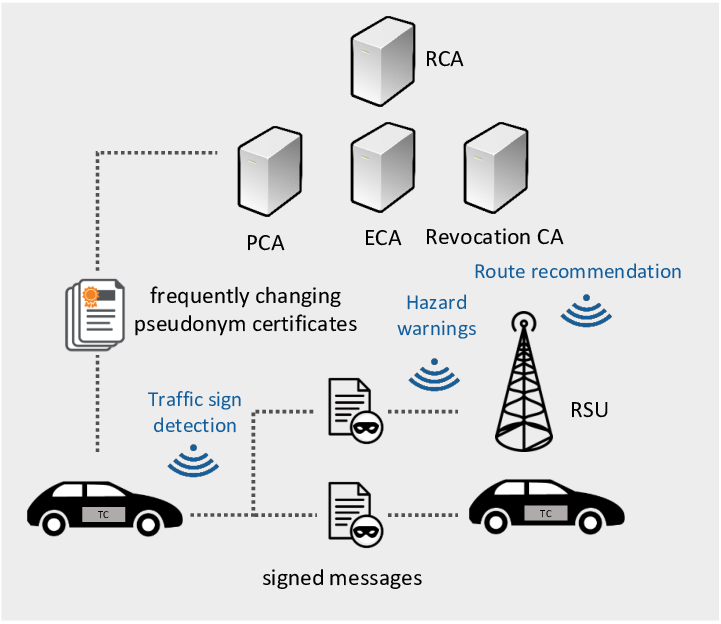
\includegraphics[width=0.88\columnwidth]{figures/rq3/rq3_vpki_security_solution_overview.png}
\caption{Overview of a V-PKI security solution: vehicles download batches of short-lived pseudonym certificates to sign safety messages without exposing permanent vehicle identities \cite{brecht2018scms}.}
\label{fig:vpki_overview}
\end{figure}

To resolve this conflict, modern Vehicular Public Key Infrastructures (V-PKIs) use \textbf{pseudonym certificates}, as shown in Fig.~\ref{fig:vpki_overview}.
Instead of using a permanent certificate on the road, a vehicle is provisioned with a large pool of temporary, short-lived pseudonym certificates that contain no personal identity information.
By regularly switching between different pseudonyms, the system provides \textit{conditional anonymity}: ordinary observers cannot link different messages to the same driver, yet authorized traffic authorities retain the mathematical ability to trace and revoke vehicles that broadcast false data.

\subsection{Trust Architecture and Multi-Authority Separation of Duties}
If a single Certificate Authority (CA) knew a vehicle's permanent identity and also issued all of its pseudonyms, an insider at that CA could easily track every car in the country.
To prevent this single point of privacy failure, modern standards enforce a strict \textbf{separation of duties} based on an honest-but-curious non-collusion model:

\begin{figure}[!t]
\centering
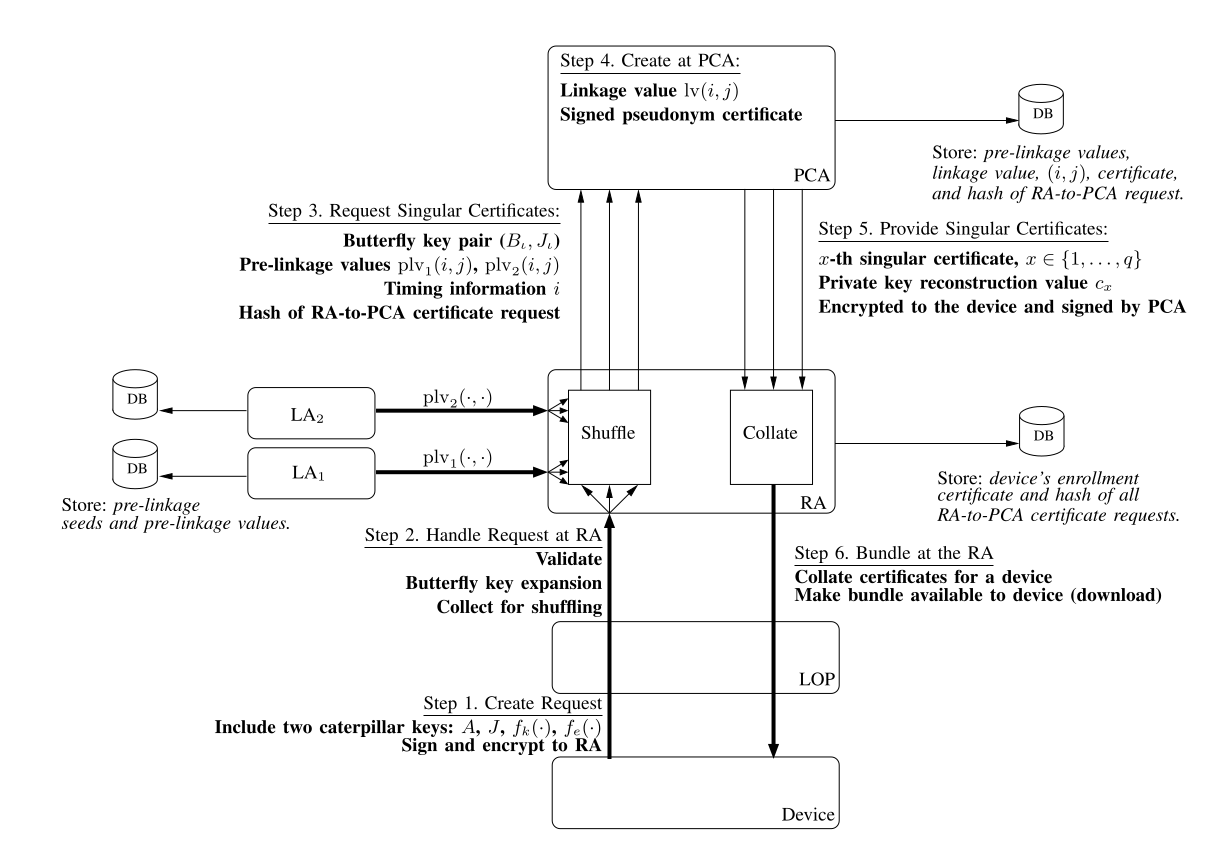
\includegraphics[width=0.95\columnwidth]{figures/rq3/rq3_scms_multi_authority_issuance_pipeline.png}
\caption{The SCMS multi-authority pseudonym issuance pipeline \cite{brecht2018scms}.}
\label{fig:scms_pipeline}
\end{figure}

\subsubsection{North American SCMS Architecture}
In the Security Credential Management System (SCMS) \cite{brecht2018scms}, backend responsibilities are divided across independent organizations, as shown in Fig.~\ref{fig:scms_pipeline}:
\begin{itemize}
    \item \textbf{Enrollment CA (ECA):} Verifies the vehicle's permanent hardware identity during manufacturing and issues a long-term enrollment certificate (its cryptographic passport).
    The vehicle never uses this certificate on the road; it only uses it to request pseudonyms.
    \item \textbf{Location Obscurer Proxy (LOP):} Acts as an anonymizing proxy that removes IP addresses and location metadata from requests before passing them to backend servers.
    \item \textbf{Registration Authority (RA):} Validates that the request comes from an authorized, non-revoked enrollment certificate.
    Crucially, the RA shuffles requests from thousands of vehicles together to break timing correlations before forwarding them to the Pseudonym CA.
    \item \textbf{Pseudonym CA (PCA):} Generates and signs the actual pseudonym certificates using compact implicit certificates.
    The PCA receives blinded requests through the RA and encrypts the resulting certificates directly for the vehicle's On-Board Unit (OBU).
    Therefore, the RA knows \textit{who} asked for certificates, and the PCA knows \textit{which} certificates were issued, but neither entity knows both.
    \item \textbf{Linkage Authorities ($LA_1$ and $LA_2$):} Two independent servers that generate pre-linkage values ($plv_1, plv_2$) embedded inside each pseudonym.
    If a car misbehaves, the XOR combination of both values ($lv = plv_1 \oplus plv_2$) allows revoking all of that car's certificates at once.
    Neither LA can link certificates on its own.
\end{itemize}

\subsubsection{European C-ITS Trust Model}
The European C-ITS architecture (ETSI TS~102~940 and TS~102~941) uses a similar functional split \cite{haidar2019risk, yoshizawa2023new}.
An Enrolment Authority (EA) manages long-term identities, while an Authorization Authority (AA) issues short-term Authorization Tickets (ATs) used as pseudonym certificates.
Long-term credentials are never broadcast over the air.

\subsection{Scalable Batch Issuance: Butterfly Key Expansion}
Vehicles often drive through rural areas or underground tunnels without cellular coverage for extended periods.
Consequently, an OBU must preload a batch of thousands of pseudonym certificates at a time (e.g., a one- to three-year supply).
However, generating and uploading thousands of individual public keys over wireless connections is prohibitively slow and consumes excessive cellular bandwidth.

\begin{figure}[!t]
\centering
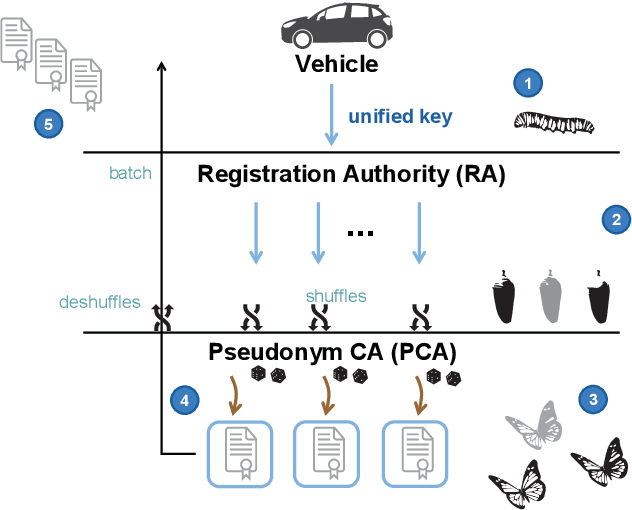
\includegraphics[width=0.88\columnwidth]{figures/rq3/rq3_butterfly_key_expansion_flow.png}
\caption{The Butterfly Key expansion process \cite{brecht2018scms}.}
\label{fig:butterfly_flow}
\end{figure}

The \textbf{Butterfly Key Expansion} mechanism solves this scalability bottleneck \cite{brecht2018scms}, as illustrated in Fig.~\ref{fig:butterfly_flow}:
\begin{enumerate}
    \item The vehicle uploads a single base public key (the \textit{caterpillar key}) to the RA along with an expansion function.
    \item The RA uses this single key to mathematically derive thousands of intermediate public keys (\textit{cocoon keys}) on the vehicle's behalf, and shuffles them across many vehicles.
    \item For each cocoon key, the PCA generates a random secret offset, adds it to the cocoon key to create the final \textit{butterfly public key}, and embeds it into a pseudonym certificate.
    \item The PCA encrypts the certificates and offsets for the vehicle and returns them through the RA.
    \item The vehicle decrypts the package, adds the PCA's secret offset to its original private seed, and reconstructs the corresponding private signing key locally.
\end{enumerate}
This process allows an OBU to obtain thousands of valid pseudonym certificates in a single compact message without the RA or PCA compromising privacy.
Earlier alternatives, such as the PASS proxy re-signature scheme \cite{sun2010efficient}, offloaded certificate generation to RSUs using bilinear pairing cryptography, but required high computation overhead.

\subsection{Revocation Mechanisms and Credential Management}
When a vehicle is compromised, hacked, or suffers a sensor malfunction, it must be revoked so other vehicles ignore its safety messages.
However, revoking pseudonym certificates is difficult: if a rogue vehicle holds 3,000 valid pseudonyms, placing every individual serial number on a traditional Certificate Revocation List (CRL) would make the CRL file huge, overwhelming wireless channels and OBU memory.

\subsubsection{Active Revocation via Linkage Values}
To keep CRLs small, SCMS embeds hash-chain Linkage Values inside each certificate \cite{brecht2018scms}.
For each time period $t$, both Linkage Authorities advance their one-way hash chains and compute pre-linkage values ($plv_1, plv_2$).
Under normal driving, the resulting Linkage Value ($lv = plv_1 \oplus plv_2$) looks like random noise to outside observers.
When a vehicle must be revoked at time period $t_s$, the authority publishes only that vehicle's two seed values for period $t_s$ on the CRL.
This requires only 48~bytes per revoked vehicle ($O(1)$ constant overhead).
Using these seeds, any receiving vehicle on the road can compute all current and future linkage values for that vehicle ($t \ge t_s$) and instantly reject its messages.
Because cryptographic hash functions are one-way, publishing seeds for period $t_s$ provides \textit{retrospective unlinkability} (backward privacy): attackers cannot reverse the hash to uncover trips the driver made before being revoked.

\subsubsection{Passive Revocation: IFAL and Automotive OAuth 2.0}
To avoid broadcasting CRLs over the air entirely, the European Issue First Activate Later (IFAL) scheme preloads dormant certificates into vehicle storage \cite{yoshizawa2023new}.
Certificates are activated in 90-day periods using small activation keys downloaded from the authority.
If a vehicle misbehaves, the authority simply stops sending future activation keys, and the vehicle is passively silenced once its current 90-day period expires.
To improve this concept and eliminate the 90-day vulnerability window, Yoshizawa and Preneel \cite{yoshizawa2023new} proposed an automotive OAuth~2.0 framework with ratcheting encryption.
Starting the vehicle's engine acts as driver consent, triggering the OBU to request daily activation tokens from the authority.
The onboard Hardware Security Module (HSM) verifies the token before unlocking signing capabilities, shrinking the revocation window down to 24~hours.

\subsection{Limitations and Practical Vulnerabilities}
Despite their sophisticated design, pseudonym systems face significant technical limitations:

\begin{figure}[!t]
\centering
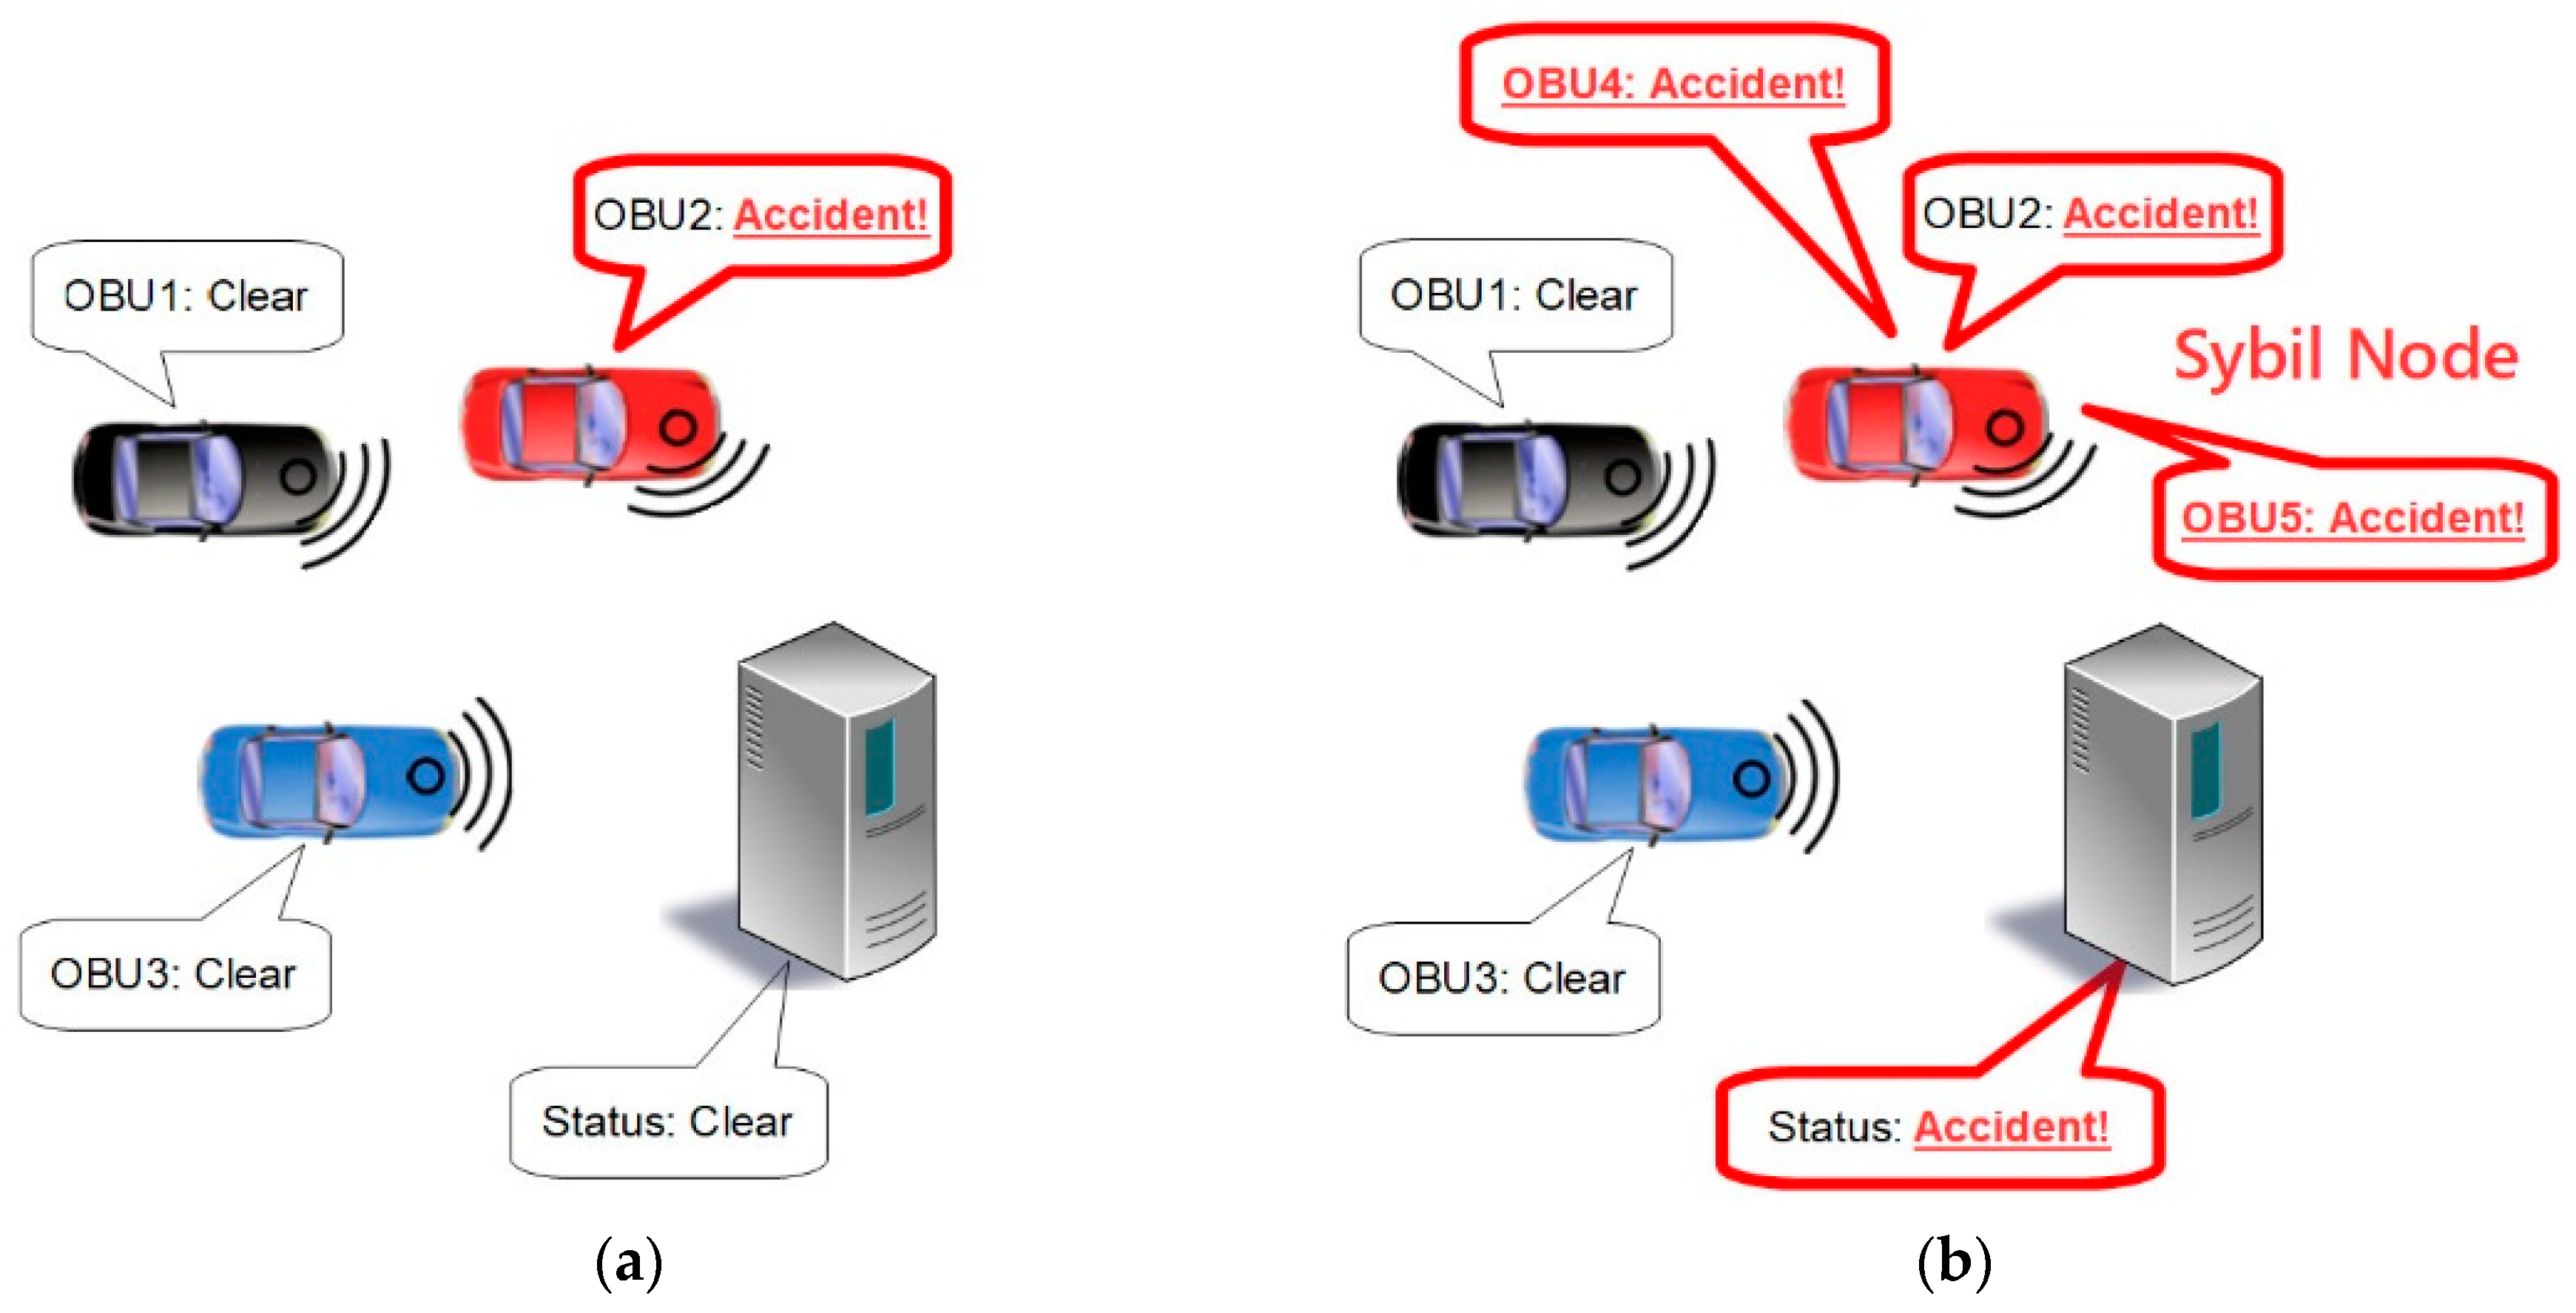
\includegraphics[width=0.92\columnwidth]{figures/rq3/rq3_sybil_attack_concurrent_pseudonyms.png}
\caption{Sybil attack exploiting concurrent pseudonym pools: (a) A single false alert is outvoted by honest vehicles; (b) A malicious node uses three valid pseudonyms simultaneously to manufacture a fake accident majority \cite{haidar2019risk}.}
\label{fig:sybil_attack}
\end{figure}

\begin{itemize}
    \item \textbf{Multi-Key Birthday Attacks:} Simplício et al. \cite{simplicio2018privacy} demonstrated that because SCMS Linkage Authorities encrypt fixed plaintexts under 128-bit keys, an attacker collecting pre-linkage values from 20,000 vehicles over a year can execute a multi-key collision attack that lowers effective security to 108~bits (below the NIST 112-bit minimum).
    This vulnerability is resolved by injecting unique 96-bit domain-separated security strings into each hashing step.
    
    \item \textbf{The Certificate Waste Paradox:} In systems that assign rigid sequential time slots to certificates, certificates expire when their time window passes.
    Because private passenger cars remain parked approximately 96\% of the time, empirical studies show that 95.2\% of all issued pseudonym certificates expire without ever signing a single message \cite{yoshizawa2023new}.
    Scaled across the European Union's 277 million vehicles, this wastes approximately 1.85 Petabytes of cryptographic data annually.
    
    \item \textbf{Sybil Attacks and Pool Exhaustion:} To reduce certificate waste, industry consortia allow vehicles to hold concurrent pools of valid certificates (e.g., 20 to 100 certificates per week).
    However, Haidar et al. \cite{haidar2019risk} showed that this introduces dangerous vulnerabilities, as depicted in Fig.~\ref{fig:sybil_attack}.
    In a Sybil attack, a hacked vehicle signs different messages using multiple valid pseudonyms at the same moment, creating phantom vehicles that fabricate fake traffic jams or manipulate traffic signals.
    Conversely, in a pool exhaustion attack, an adversary records and replays a target vehicle's pseudonym; the victim assumes an ID collision occurred, switches certificates, and rapidly burns through its entire week's certificate budget in seconds.

    \item \textbf{Verification Latency Bottlenecks:} In pairing-based schemes like PASS \cite{sun2010efficient}, verifying a single unfamiliar certificate requires multiple bilinear pairing operations taking $\approx 14.7$~ms.
    In dense highway traffic with dozens of vehicles broadcasting at 10~Hz, the message processing queue overflows, dropping 40\% to 50\% of incoming safety packets.
    For this reason, standard V-PKIs mandate hardware-accelerated ECDSA signatures.

    \item \textbf{Syntactic versus Semantic Privacy:} Pseudonym certificates provide only syntactic privacy (changing the digital signature and header ID).
    They provide zero semantic privacy over the physical trajectory data inside the packet.
    Because safety beacons broadcast exact GPS positions ten times per second, an eavesdropper using standard Kalman filters can easily connect consecutive beacons across pseudonym switches based on vehicle speed and heading \cite{brecht2018scms}.
    To break this physical tracking, pseudonym changes must be combined with physical Pseudonym Change Strategies (PCS), such as intersection Mix-Zones (Fig.~\ref{fig:mix_zone}) or silent periods during lane changes.
\end{itemize}

\begin{figure}[!t]
\centering
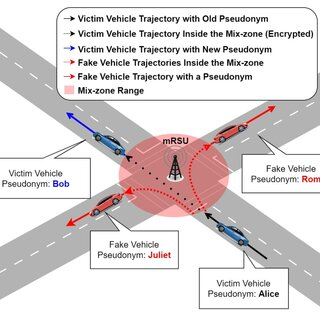
\includegraphics[width=0.72\columnwidth]{figures/rq3/rq3_mix_zone_intersection_pseudonym_change.jpg}
\caption{Mix-zone deployment at an intersection: encrypting beacons and injecting decoy trajectories inside the mix-zone prevents external trackers from linking entry pseudonyms to exit pseudonyms.}
\label{fig:mix_zone}
\end{figure}
